\documentclass[a4paper,14pt,oneside,openany]{memoir}
\usepackage{coursework}
    
% Информация для титульного листа и листа задания
% Следует заполнить актуальными данными

% Кафедра, на которой читается дисциплина
\setdepartment{Электронно-вычислительные машины и системы}

% Инициалы и фамилия заведующего кафедрой
\setdepartmentchairname{А.Е.~Андреев}

% Полное название дисциплины
\setsubject{Системы обработки больших данных}

% Название темы курсовой работы
\settheme{Исследование датасета атмосферных осадков в Гонконге с использованием фреймворка Apache Spark}

% Фамилия Имя Отчество студента
\setstudentname{Иванов Иван Иванович}

% Инициалы и фамилия студента
\setstudentinitials{И.И.~Иванов}

% Учебная группа студента
\setgroupname{ЭВМ-1.1}

% Инициалы и фамилия преподавателя, проверяющего курсовую работу
\setadvisorname{П.Д.~Кравченя}


\begin{document}

\maketitlepage % Создаем титульный лист

\renewcommand{\contentsname}{Содержание}
\tableofcontents*
\addtocontents{toc}{\vspace{1\baselineskip}}
\clearpage

\justifying
\chapter*{Введение}
\addcontentsline{toc}{chapter}{\MakeUppercase{Введение}}
\vspace{\baselineskip}

% Содержание введения
%
Во введении сначала дается краткая характеристика области, в которой выполнена работа (1 -- 3 предложения). Затем обосновывается актуальность работы.

Далее идут фразы, которые лучше повторить дословно:

В связи с этим целью данной работы являлось ... (цель должна быть одна).

Для достижения поставленной цели решались следующие задачи:
\begin{enumerate}
    \item первая задача;
    \item вторая задача;
    \item третья задача;
    \item ...
\end{enumerate}

В конце введения следует добавить описание структуры курсовой работы. Например:

В первом разделе рассмотрена более подробно постановка задачи и проведен обзор литературы по ... Во втором разделе ... В третьем разделе ... В заключении работы сформулированы общие выводы ...

% Здесь пишется содержание первой главы
%
\chapter{\MakeUppercase{Разведочный анализ данных с использованием PySpark}}\label{ch:first}
\section{Постановка задачи разведочного анализа}\vspace{\baselineskip}

Здесь нужно сформулировать постановку задачи разведочного анализа: что дано, и что нужно сделать.

\vspace{\baselineskip}\section{Описание датасета}\vspace{\baselineskip}

Здесь требуется описать выбранный датасет, привести ссылку на него, охарактеризовать его тематику, объем, количество признаков. Вкратце нужно описать признаки датасета (допускается описывать не все признаки, а только те, которые используются в исследовании).
Также, можно сослаться на источники, например, в \cite{karau2015spark, koirala2020pyspark, white2013hadoop, Tekdogan2022} рассматривается материал об ... Часть информации можно оформить в виде таблицы, но избегайте слишком длинных таблиц. На каждую таблицу должна быть ссылка в тексте, как, например, на таблицу \ref{tab:features}, в которой приведен пример описания признаков.

\begin{table}[]
    \centering
    \begin{tabularx}{\textwidth}{|X|X|}
        \hline
        \multicolumn{1}{|c|}{Признак}  & \multicolumn{1}{c|}{Расшифровка признака}   \\ \hhline{|=|=|}
        Temperature                    & Среднемесячная температура в \degree C      \\ \hline
        Humidity                       & Влажность в процентах                       \\ \hline
    \end{tabularx}
    \caption{Пример таблицы признаков}
    \label{tab:features}
\end{table}

\vspace{\baselineskip}\section{Определение пропущенных значений}\vspace{\baselineskip}

Обратите внимание, что приведенная здесь структура раздела не является жестким требованием, а служит примером оформления. При необходимости, её можно корректировать в разумных пределах.

При необходимости можно вставить рисунок и сослаться на него: на рисунке \ref{fig:HadoopEcoSystem} приведена иллюстрация экосистемы Hadoop. Обратите внимание, что таблицы и рисунки являются <<плавающими>> объектами: они могут располагаться не в месте их непосредственного объявления, а в некоторой близости от него.

\begin{figure}
    \centering
    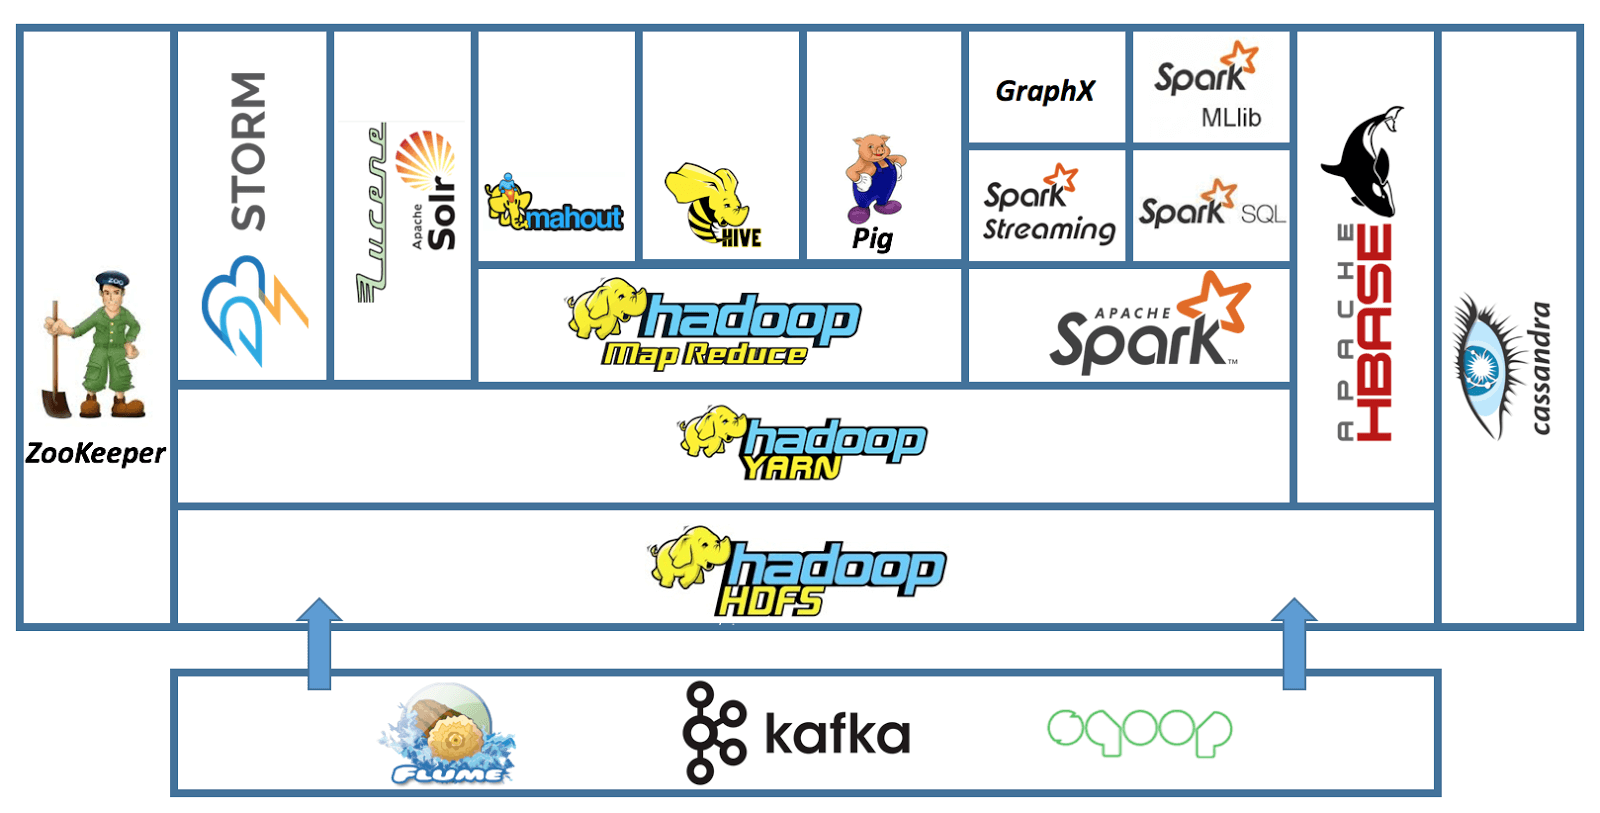
\includegraphics[width=\textwidth]{Content/Images/HadoopEcoSystem.png}
    \caption{Иллюстрация экосистемы Hadoop}
    \label{fig:HadoopEcoSystem}
\end{figure}

Также, вот пример списка:

\begin{itemize}
    \item первый элемент;
    \item второй элемент;
    \item третий элемент;
    \begin{itemize}
        \item вложенный элемент.
    \end{itemize}
\end{itemize}

А здесь -- аналогичный нумерованный список:

\begin{enumerate}
    \item первый элемент;
    \item второй элемент;
    \item третий элемент;
    \begin{enumerate}
        \item вложенный элемент.
    \end{enumerate}
\end{enumerate}

А вот формула, которая связывает между собой синус, косинус и тангенс.

\begin{equation}
    \label{eq:formula}
    \tg \alpha = \frac{\sin \alpha}{\cos \alpha}.
\end{equation}

Ну, и ссылка на неё: формула (\ref{eq:formula}) выражает связь тригонометрических функций.

\vspace{\baselineskip}\section{Другая подглава}\vspace{\baselineskip}

Здесь можно продемонстрировать пример включения фрагмента кода в текст работы. И заодно добавить еще пару ссылок \cite{spark2022official, zaharia2021lakehouse}.
\begin{code}
import matplotlib.pyplot as plt
import numpy as np
x = np.linspace(0, 10, 100)
y = np.sin(x)
plt.figure(figsize=(10, 6))
plt.plot(x, y, label='sin(x)', color='blue', linewidth=2)
plt.title('График функции sin(x)', fontsize=16)
plt.xlabel('x', fontsize=14)
plt.ylabel('sin(x)', fontsize=14)
plt.legend()
plt.grid(True)
plt.show()    
\end{code}

Здесь продолжается текст. Не забывайте, что фрагмент кода не должен превышать половины страницы -- затем должен следовать текст.

\vspace{\baselineskip}\section{Выводы}\vspace{\baselineskip}

В конце каждой главы должны быть выводы. Они представляют собой несколько предложений, которые кратко характеризуют проделанную в главе работу и полученные результаты.


% Здесь пишется содержание второй главы
%
\chapter{\MakeUppercase{Машинное обучение на больших данных}}\label{ch:second}

\vspace{\baselineskip}
При необходимости, в главу можно добавить преамбулу с кратким введением в содержание этой главы.
\vspace{\baselineskip}

\section{Задача регресии}
\subsection{Постановка задачи регрессии}\vspace{\baselineskip}

Здесь нужно сформулировать поставленную задачу регрессии, которая будет решаться дальше.

\vspace{\baselineskip}\subsection{Решение задачи регрессии}\vspace{\baselineskip}

Здесь подробно описывается решение задачи регрессии.

\vspace{\baselineskip}\subsection{Анализ полученных результатов}\vspace{\baselineskip}

После решения задачи и получения результатов их необходимо проинтерпретировать.

\vspace{\baselineskip}\section{Задача бинарной классификации}
\subsection{Постановка задачи бинарной классификации}\vspace{\baselineskip}

Аналогично задаче регрессии.

\vspace{\baselineskip}\subsection{Решение задачи бинарной классификации}\vspace{\baselineskip}

Аналогично задаче регрессии.

\vspace{\baselineskip}\subsection{Анализ полученных результатов}\vspace{\baselineskip}

Аналогично задаче регрессии.

\vspace{\baselineskip}\section{Выводы}\vspace{\baselineskip}

Сформулированные выводы по главе.


% Здесь пишется содержание третьей главы
%


% Здесь пишется содержание четвёртой главы
%


\chapter*{Заключение}
\addcontentsline{toc}{chapter}{\MakeUppercase{Заключение}}
\vspace{\baselineskip}

% Здесь пишется заключение по работе
%
В заключении коротко приводятся и анализируются полученные результаты, предлагаются дальнейшие направления развития темы.

\clearpage

\printbibliography

%%% Настройки для приложений
\appendix

% Оформление заголовков приложений ближе к ГОСТ:
\renewcommand*{\printchaptername}{\MakeUppercase{\appendixname}}
\renewcommand*{\afterchapternum}{\centering\par\nobreak\vskip \midchapskip}
\renewcommand*{\printchapternum}{\chapnumfont \thechapter}
\renewcommand\thechapter{\Asbuk{chapter}}
\renewcommand*{\printchaptertitle}[1]{\chaptitlefont #1}

% Здесь пишется содержание приложений
%
\chapter{Пример листинга программного кода}\label{app:A}\vspace{\baselineskip}

Здесь можно привести полный листинг кода программы или модуля.

\begin{code}
import matplotlib.pyplot as plt
import numpy as np

# Данные для графика
x = np.linspace(0, 10, 100)
y = np.sin(x)

# Создание графика
plt.figure(figsize=(10, 6))

plt.plot(x, y, label='sin(x)', color='blue', linewidth=2)

# Настройка графика
plt.title('График функции sin(x)', fontsize=16)
plt.xlabel('x', fontsize=14)
plt.ylabel('sin(x)', fontsize=14)
plt.legend()
plt.grid(True)

# Вывод графика
plt.show()    
\end{code}

\chapter{Пример второго приложения}\label{app:B}\vspace{\baselineskip}

При необходимости, приложений может быть несколько.


\end{document}
